\chapter{Measurements}
\label{cha:measurements}
For measuring different simulation designs a example network was implemented using a monolithic and a modular design.
The simulation of this network using the different designs is used for analyzing the impact of the design on the performance.
This network simulates a message queue with different types of transmitted data (configuration, event, historical).
The different types of data are processed by different parts within the network.
This network includes different parts which generate data and process data.
The simulated network is shown in Figure \ref{fig:design_test_network}.

\begin{figure}
    \centering
    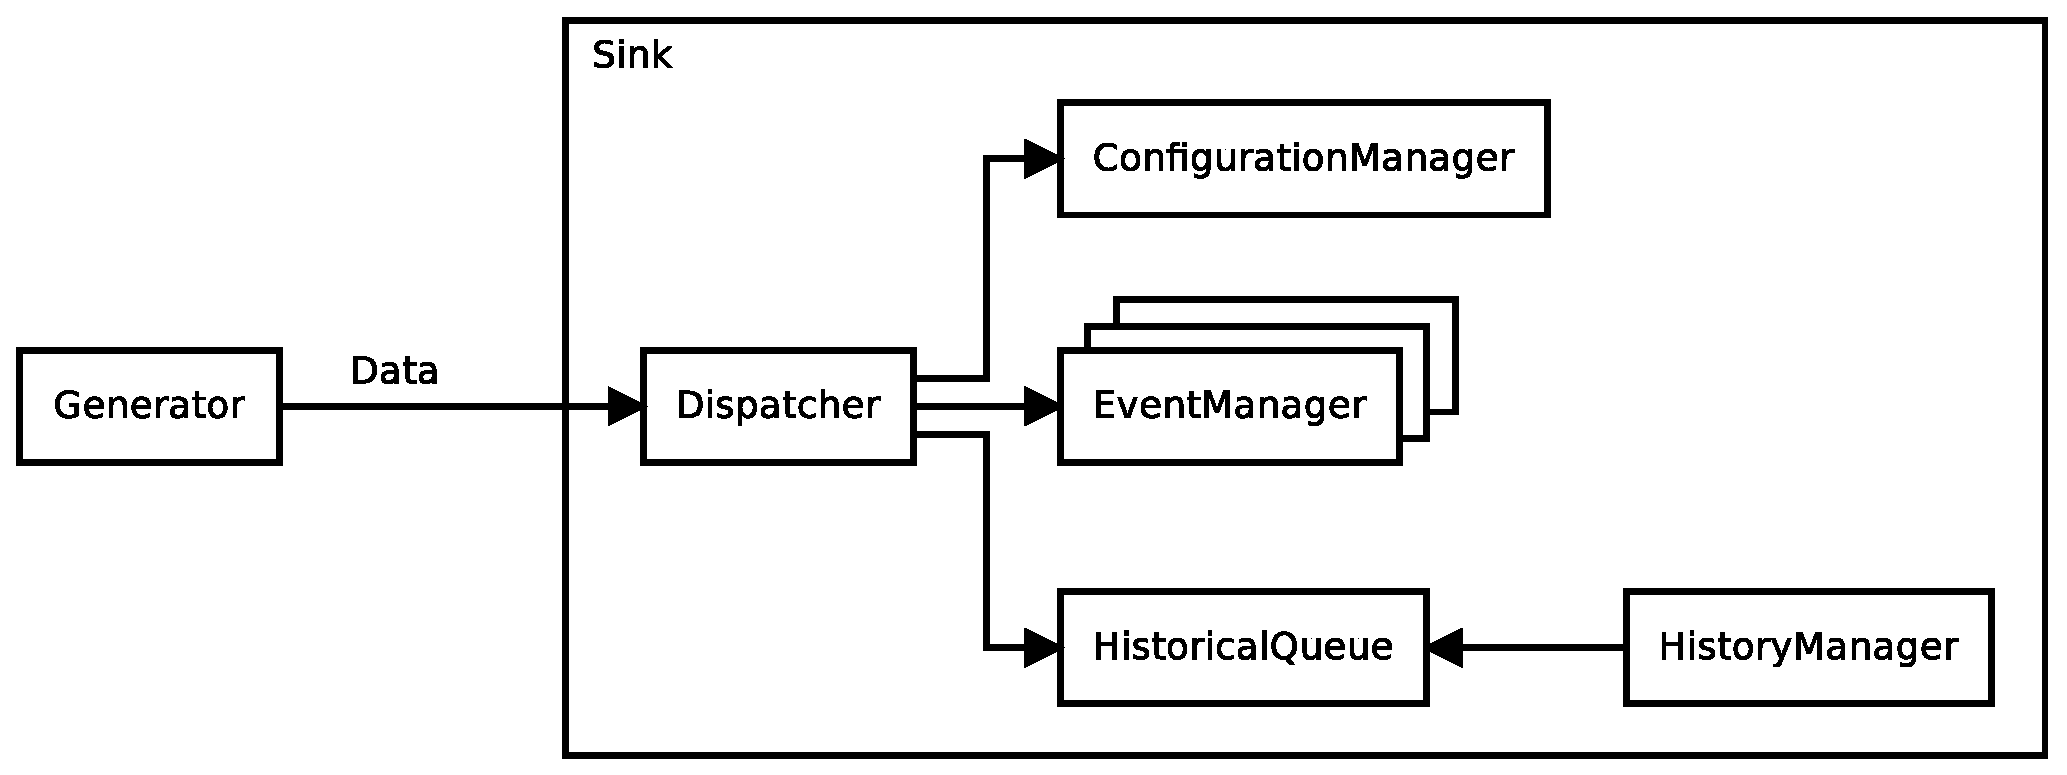
\includegraphics[width=0.9\linewidth]{design_test_network.eps}
    \caption{Example network including generator, sink, queue and different manager.}
    \label{fig:design_test_network}
\end{figure}

The \emph{Generator} generates cyclic data and a polling command.
Both are transmitted via messages to the sink module
The generated data includes a field of 64 Bytes and a enumeration describing the type of data.

\section{Simulated example network}
\label{sec:measurements_network}
This data is transmitted to a sink, which is described via the interface module \emph{ISink}.

The differently designed modules \emph{ModularSink} and \emph{MonolithicSink} extend the interface and represent the different tested designs.

The first part within the sink is the \emph{Dispatcher} which is accessing the type information of the data and then forwards the packed data to the according parts.
Configuration and event data are forwarded to the \emph{ConfigurationManager} and the \emph{EventManager}.
These parts are simple implementations which executes various calculations on the received data to simulate processing.

Historical data are forwarded to the \emph{HistoricalQueue} which is internally implemented by a std::queue which holds all received data until they are accessed.
The \emph{HistoryManager} accesses the \emph{HistoricalQueue} and processes available data.
This access is initiated by the generated polling commands from the \emph{Generator}.
\\

The functionality of dispatching and processing of the data is, as shown in Figure \ref{fig:design_test_network}, is included in the sink and is implemented twice with different designs.


Given the implementation of the different parts of the targeted functionality, implementing the \emph{MonolithicSink} consists of instantiating and connecting the different parts within a single simple module.

The received messages will be forwarded to the different parts according to the input gate.

Implementing the \emph{ModularSink} requires the implementation of wrapper modules for every single part which should be represented by a separate module.
These wrapper extract the transmitted data of received messages and forward it to the enclosing parts.
Calls from within the enclosed parts are handled by methods of the wrappers, which are passed via function pointers (functional objects).
Within this methods according messages are created and sent via output gates.

\section{Measurement methods}
\label{sec:measurements_methods}
For measuring the performance of the different designs three measurement methods was implemented.

\subsection{Runtime measurement}
\label{sec:measurements_methods_runtime}
The performance of the simulated design can be analyzed by defining a fixed simulation time limit (\emph{sim-time-limit}).
Using the default (non real-time) scheduler this results in a simulation which executes as fast as possible the needed number of event for reaching the simulation time limit.
The required time for this simulation represents the performance of the simulation.

\subsection{Processed event count}
\label{sec:measurements_methods_event}
By defining a fixed execution time limit (\emph{cpu-time-limit}) and using the default scheduler the simulation will run for a fixed time.
The number of processed events within this fixed time represents the performance of the simulation.
The simulation of different designs results in contrasting event counts due to the increased number of messages within a modular design.
Therefore for evaluating the created number within a fixed processing time the ratio of event creation must be determined.
This ratio can be measured using the previous method.

\subsection{Real time behavior}
\label{sec:measurements_methods_realtime}
Using the built in real time scheduler \emph{cRealTimeScheduler} the simulation will try to execute the simulation matching the real time.
The performance output (\emph{cmdenv-performance-display}) provides the ratio of simulated seconds per real second.
As described in section \ref{sec:simulation_real_time} this ratio must not differ too much from one for representing a real-time simulation.
The simulated network provides a configurable interval of data/command generation.
Using a parameter study (described in section \ref{sec:omnet_running_config}) the interval for data/command generation can be set with values form a range of intervals.
With attention to the performance ratio of the different iterations the interval limit, which still allows real-time simulation, can be determined.

\section{Sequential Simulation}
\label{sec:measurements_sequential}

\section{Parallel simulation}
\label{sec:measurements_parallel}